\section{Purpose of the Task Dataset}
The simulator does not ingest radiance measurements or images. It ingests a task table in which each row represents a fire region that may justify a follow-up observation. Building that table requires a decision about which thermal detections describe the same event. Keeping every pixel creates repeated requests for one fire; merging too broadly removes distinct events. The final pipeline therefore retains source-product references and applies de-duplication before architecture evaluation.

Two three-day event windows are used. California covers 3-5 July 2025 and includes the early stage of the Madre Fire. India covers 14-16 April 2026 and represents a much denser workload. These windows are engineering cases, not a statistical sample of global fire behaviour. California contains 32 final tasks; India contains 773. A regional difference consequently combines event selection, geography, timing, density, and priority composition. It is described as a workload contrast, not a pure geographic effect.

Figure~\ref{fig:task_map} places every retained task on a geographic boundary rather than on an empty coordinate grid. The California outline comes from the US Census Bureau cartographic boundary files and the India outline from Natural Earth \citep{USCensus2025Boundaries,NaturalEarth2025}. The study-region filter uses event bounding boxes, so a small number of retained coordinates may fall outside the political boundary; the map makes that selection effect visible rather than clipping those tasks.

\begin{figure}[htbp]
\centering
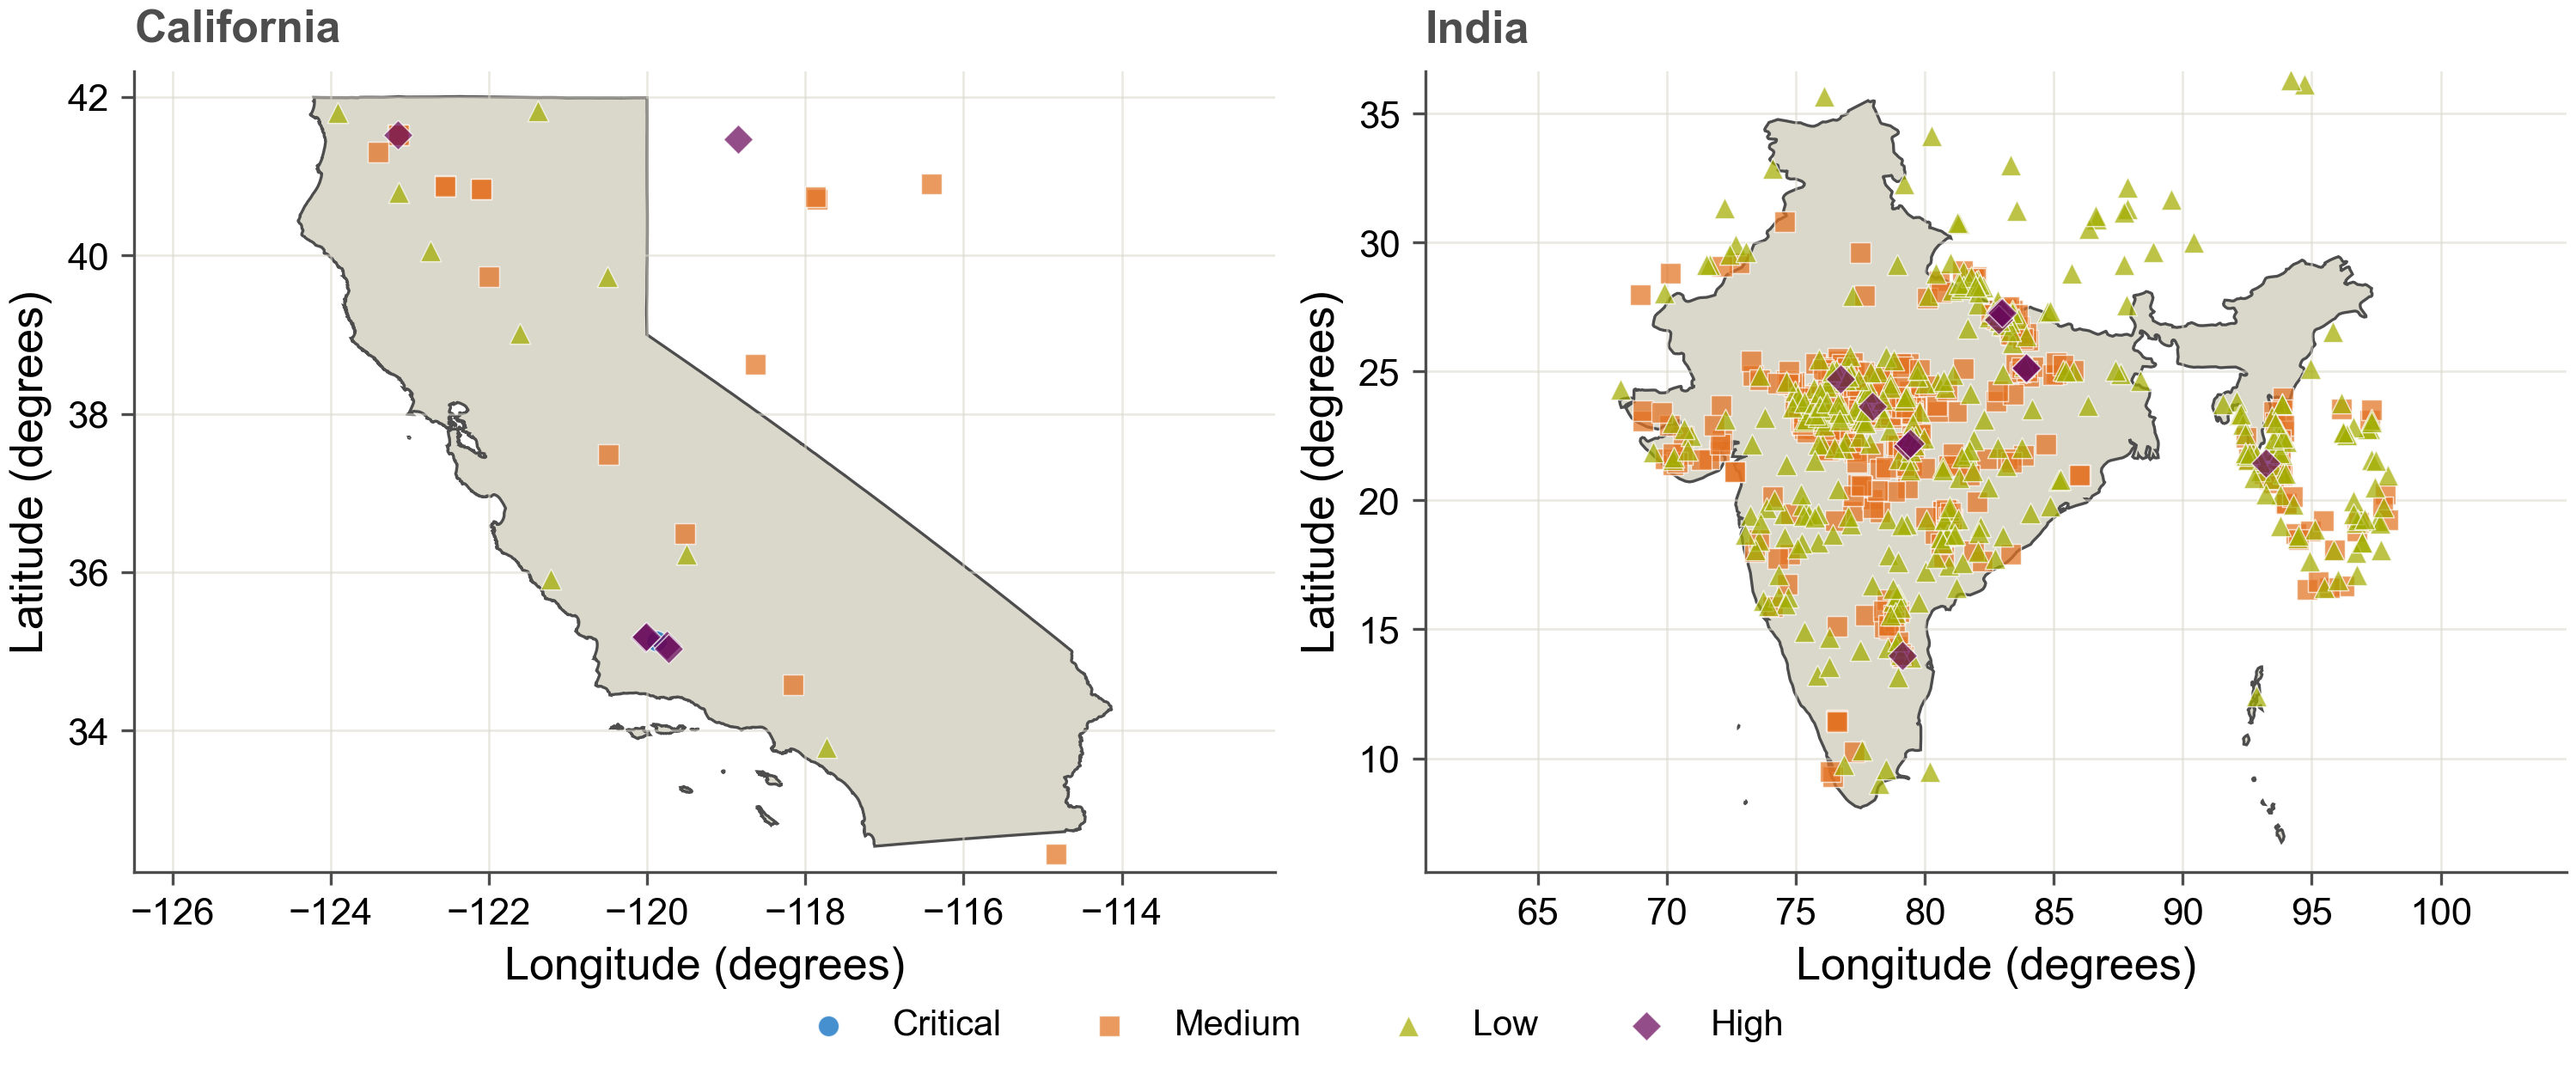
\includegraphics[width=0.96\textwidth]{figures/part1_revision/task_map.png}
\caption{Geographic distribution of all 805 final Sentinel-3 tasks on published administrative outlines. California contains 32 tasks and India 773; marker shape and colour identify the priority class.}
\label{fig:task_map}
\end{figure}
\section{Processing Sequence}
Figure~\ref{fig:task_pipeline} summarizes the implemented path from product records to simulator input. The purpose of each stage is different: filtering defines the sample, clustering forms candidate fire regions, scoring creates an engineering priority, and de-duplication determines which candidates remain independent tasks.

\begin{figure}[htbp]
\centering
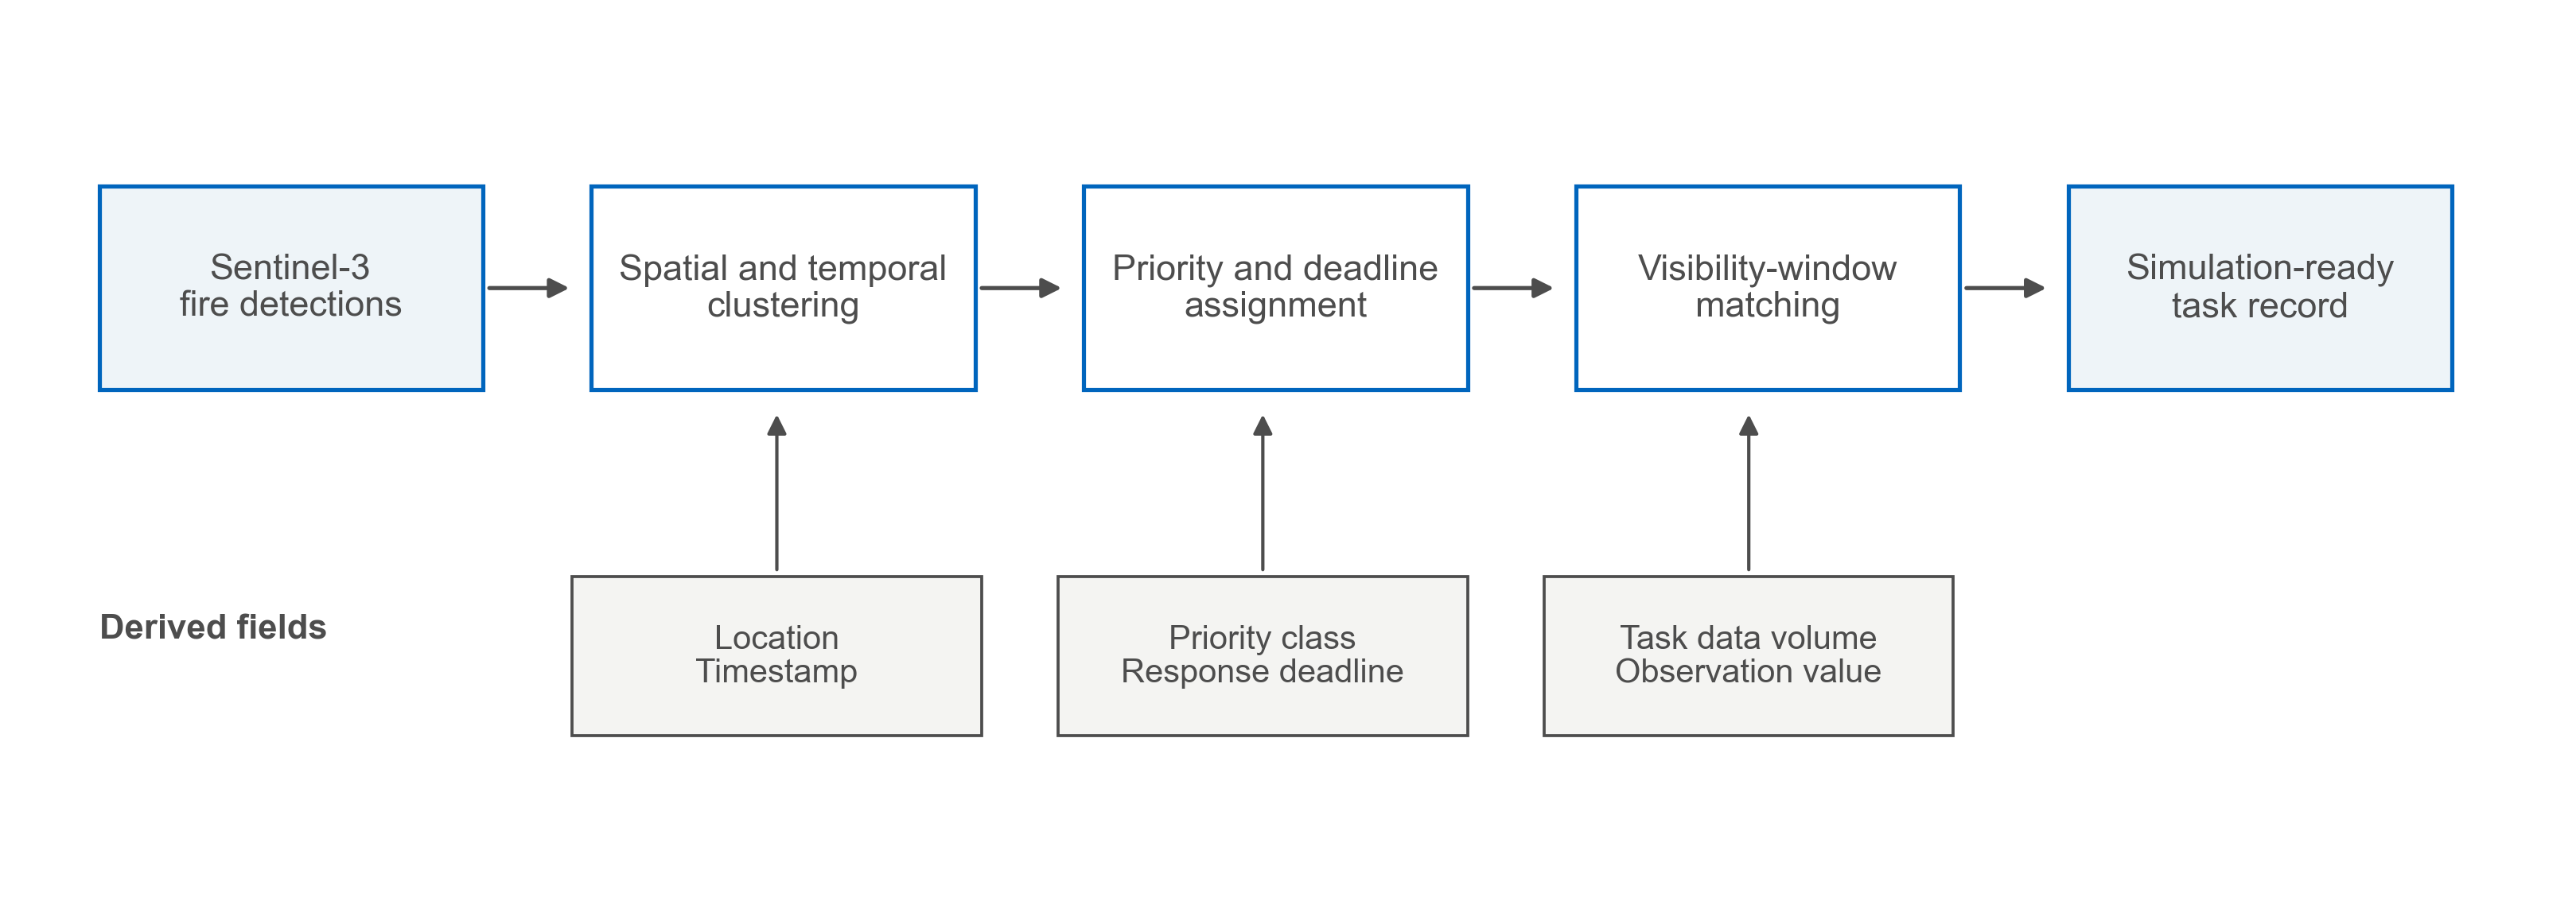
\includegraphics[width=0.96\textwidth]{figures/part1_revision/task_pipeline.png}
\caption{Traceable task-generation workflow. Filtering occurs before clustering, and the exported task retains source-product provenance.}
\label{fig:task_pipeline}
\end{figure}
Each downloaded \texttt{.SEN3} directory represents one Sentinel-3 SLSTR Level-2 FRP granule. The sensing interval is read from the product record. Geolocated fire pixels are extracted from the primary FRP NetCDF file, filtered by event window and region, and checked for valid coordinates and FRP. Product identifiers remain attached to the resulting task so a simulated row can be traced back to its source.

De-duplication is applied at four levels:

\begin{enumerate}
\item Each Sentinel-3 product is read once.
\item Only the primary FRP NetCDF content is used for fire pixels.
\item Exact and near-duplicate hotspot rows are removed using position, time, and FRP.
\item Candidate tasks that represent the same fire region on the same day are merged, retaining a traceable representative and the strongest priority evidence.
\end{enumerate}
The reduction in reported FRP during pipeline development reflects removal of repeated records; it is not evidence of a physical decrease in fire activity.

\section{FRP Filtering and DBSCAN Clustering}
The development pipeline applies an FRP inclusion threshold of 10 MW before spatial grouping. This threshold is an engineering rule for generating communication tasks, not a definition of wildfire occurrence.

Density-Based Spatial Clustering of Applications with Noise (DBSCAN) is used because the number of fire regions is not known in advance. DBSCAN connects detections that have enough neighbours within a chosen distance. Here, \texttt{eps} is the neighbourhood radius and \texttt{min\_samples} is the minimum number of detections required for a dense cluster. The documented baseline uses a 10 km neighbourhood and \texttt{min\_samples = 3}.

The sequence is important. The date, region, quality, and FRP filters are applied first. DBSCAN is then run on the retained positions for the declared grouping unit. Dense detections become a cluster; isolated points follow the explicit noise-point rule rather than being silently attached to the nearest cluster. Each exported task retains its centroid, approximate radius, number of contributing detections, and product provenance. Table~\ref{tab:task_population} therefore describes the final output after filtering and de-duplication, not the number of raw fire pixels.

The clustering choice controls network load. A smaller radius creates more packets and can fragment one event. A larger radius creates fewer packets and can merge independent events. The baseline must therefore be interpreted together with the proposed 5 km and 20 km sensitivity checks.

\section{Confidence and Priority}
Sentinel-3 supplies numerical MWIR confidence information. FIRMS VIIRS uses categorical low, nominal, and high values. FIRMS confidence is used only during screening and is mapped to 0.33, 0.66, and 1.00 for visualization or contextual comparison. The final simulation score uses the Sentinel-3-derived value. It is a relative ranking input, not a calibrated probability of wildfire.

Invalid Sentinel-3 confidence values are flagged as missing. A neutral value of 0.50 is used in the score so that an unavailable field does not automatically suppress the task. The missing fraction and the original confidence summaries remain in the exported data.

The FRP component combines normalized total and maximum FRP:

\begin{quote}\texttt{S\_FRP = 0.60 * N(log(1 + FRP\_total)) + 0.40 * N(log(1 + FRP\_max)).}\end{quote}
The task score is:

\begin{quote}\texttt{S\_task = 0.50 * S\_FRP + 0.30 * S\_conf + 0.20 * S\_cluster.}\end{quote}
The notation is used consistently: \texttt{S\_FRP} is the intensity term, \texttt{S\_conf} the confidence term, \texttt{S\_cluster} the spatial-support term, and \texttt{S\_task} the final score. The weights express an engineering preference for energetic strength while retaining confidence and spatial support. They were not fitted to emergency-service labels and must not be interpreted as an official severity model.

\section{Final Task Population and Packet Assumptions}
\begin{table}[htbp]\centering\small
\caption{Final Sentinel-3 wildfire-task population after filtering and de-duplication.}
\label{tab:task_population}
\begin{tabularx}{\textwidth}{XXXXXX}
\toprule
\textbf{Region} & \textbf{Critical} & \textbf{High} & \textbf{Medium} & \textbf{Low} & \textbf{Total} \\
\midrule
California & 1 & 6 & 16 & 9 & 32 \\
India & 0 & 11 & 395 & 367 & 773 \\
Total & 1 & 17 & 411 & 376 & 805 \\
\bottomrule
\end{tabularx}
\end{table}
India contributes 96 percent of all tasks, while urgent classes form a larger share of the California set. For this reason the results report both total communication volume and per-task quantities.

Priority determines the nominal response deadline and the size of the request message:

\begin{table}[htbp]\centering\small
\caption{Priority-dependent deadline and task-message size assumptions.}
\label{tab:priority_packet}
\begin{tabularx}{\textwidth}{XXXX}
\toprule
\textbf{Priority} & \textbf{Deadline} & \textbf{Packet size} & \textbf{Interpretation} \\
\midrule
Critical & 30 min & 2.0 Mbit & Immediate high-severity follow-up request \\
High & 60 min & 1.5 Mbit & Urgent follow-up request \\
Medium & 180 min & 1.0 Mbit & Time-sensitive routine request \\
Low & 360 min & 0.5 Mbit & Lower-urgency monitoring request \\
\bottomrule
\end{tabularx}
\end{table}
These sizes represent structured requests, associated metadata, and protocol allowance. They are not image products. The values are author-defined engineering assumptions chosen to create a priority-dependent capacity load while remaining small enough for UHF store-carry-forward operation. Because deadline and packet size both change with priority, the controlled size experiment holds task identity and deadline fixed and multiplies every packet by 0.5, 1, 2, or 4. This separates data-volume sensitivity from urgency.

\section{Dataset Validation and Limits}
The Madre Fire provides one event-level check. Sentinel-3 and FIRMS both place strong detections near the reported event during the California window. This check supports the geographic and temporal plausibility of the selected California task; it does not validate every task, calibrate the priority score, or measure wildfire-classification accuracy. Equivalent named-incident traceability was not established for the entire India set.

Further limits remain. Bounding boxes can retain detections outside a political boundary. Cloud, smoke, sampling, and overpass time affect which hotspots appear. FIRMS and Sentinel-3 totals are not directly comparable without spatial-temporal matching. Another sensor, season, event mix, threshold, clustering rule, or priority mapping could change the workload and the preferred architecture.

The task table is frozen before the architecture sweep. Every case within an event window therefore receives the same release times and task definitions. This makes architecture comparisons controlled within a region. It does not turn the two selected windows into population-level evidence for California or India.
